\section{Fundamentos y herramientas\label{FunAndTools}}

En esta sección vamos a realizar una breve introducción al Big Data y haremos un estudio de las herramientas que escogemos para entender mejor por qué se han seleccionado.\par

\subsection{Qué es el Big data\label{WhatIsBigD}}

El motivo por el que se inició este nuevo paradigma “Big Data” fue debido a la gran explosión de datos que tiene lugar con el surgimiento de tecnologías como la Web 2.0, los smartphones e IoT. Se calcula que se emiten más de 30 Terabytes de información cada segundo en el mundo \cite{BD-2} y el IDC predice que desde 2010 a 2020 el volumen de datos aumentará por 50 llegando por encima del Zettabyte de datos \cite{BD-2}. Por tanto, este nuevo paradigma surge debido a que los paradigmas tradicionales no tenían la capacidad de dar una respuesta al manejo de grandes volúmenes de datos.\par

En 2001, Doug Laney describe el Big Data mediante los siguientes términos conocidos como las 3 Vs del Big Data \cite{BD-4}:

\begin{itemize}
\item Volumen: El conjunto de datos debe ser grande.
\item Velocidad: Debe existir una forma rápida de que lleguen los datos, procesarlos y devolverlos.
\item Variedad: Los datos pueden ser de cualquier tipo ya sea alfanumérico, imágenes, sonidos, videos, etc…
\end{itemize}

No obstante, a día de hoy, IBM introdujo la cuarta V del Big Data que se define como Veracidad, es decir, que los datos sean lo más reales posible, ya que cuando manejamos esta cantidad de datos, encontrar datos erróneos se hace más probable. Esto quiere decir que en Big Data nos encontramos el gran reto de gestionar gran cantidad de datos de una forma óptima \cite{BD-5}.\par

Por otra parte, encontramos tres formas de tratar los datos según las diferentes necesidades que aparecen. A la hora de analizar los datos debemos tener en cuenta si se procesarán los datos del pasado, lo que implicaría reportes analíticos, entre otras aplicaciones; si se procesan en tiempo real, lo que quiere decir que se debe mostrar lo que pasa en el momento, y si queremos saber lo que pasará en el futuro, lo que implica procesos de machine learning entre otros \cite{BD-3}.\par

Por otro lado, encontramos un cambio sustancial en las herramientas que pertenecen a este paradigma. Esto ha dado lugar a las siguientes características que hecho tan popular el concepto de Big Data \cite{BD-6}: 
\begin{itemize}
	\item Las bases de datos manejan datos no estructurados, aportando mucha más flexibilidad y dando lugar a las bases de datos NoSQL.
	\item El hecho de almacenar los datos en una sola máquina suponía un mayor gasto económico y dificultad en su propia administración, lo que supuso que surgiera el concepto de escalabilidad horizontal de los datos. Este concepto implica que los datos no aparecen en una sola máquina, sino que se distribuyen horizontalmente entre varias máquinas. Para añadir seguridad a estas bases de datos distribuidas, debe existir una redundancia de datos que son repartidos en cada máquina, dando lugar a que cada una de ellas tenga una pequeña copia de otra para poder recuperarse.
	\item Siguiendo con el punto anterior, se debe escalar horizontalmente el procesamiento de los datos. Esto implica una coordinación absoluta entre las diferentes máquinas que alojan los datos y los procesan para devolverlos procesados a un nodo líder del cluster y que sea capaz de devolver, rápidamente, los datos procesados.                   
	\item Finalmente, tras obtener los datos, los usuarios desean que se pueda visualizar fácilmente la información recogida. Para que dicha cantidad de datos, sea más fácil de entender, se pueden mostrar en diferentes gráficas aplicando diversas ecuaciones estadísticas significativas si fuera necesario. El hecho de que este paradigma maneja gran cantidad de datos a favorecido el desarrollo de herramientas de visualización de datos. 
\end{itemize}

\subsection{Docker\label{Docker}}


Docker es un proyecto OpenSource que nos ayudará, de una forma eficiente, simple, segura, portable y replicable a lanzar servicios \cite{Dck-5} \cite{Dck-6}. Para entender Docker, debemos entender el concepto de contenedor. Según la definición que nos da RedHat, un contenedor es:\par
\begin{quote}

\small ``Un contenedor de Linux es un conjunto de procesos que están separados del resto del sistema, que se pueden ejecutar desde una imagen diferente que proporciona todos los archivos necesarios para dar soporte a los procesos. Al proporcionar una imagen que contiene todas las dependencias de una aplicación, es portátil y consistente mientras cambia de la etapa de desarrollo a la de prueba y, finalmente, a la de producción."\cite{Dck-7}\par

\end{quote}
En definitiva, un contenedor, a diferencia de una máquina virtual, no tiene que usar la capa del sistema operativo y esto hace que tampoco necesite el hypervisor. Por tanto, un contenedor es capaz de lanzar diferentes aplicaciones y librerías sobre la capa del sistema operativo que las aloja de una forma aislada y segura permitiendo, además, un arranque mucho más rápido, ya que no tiene que cargar la imagen del SO. Esto lo podemos ver en la figura \ref{dock-1} \cite{Dck-7}.\par

\begin{figure}[htp]
\centering
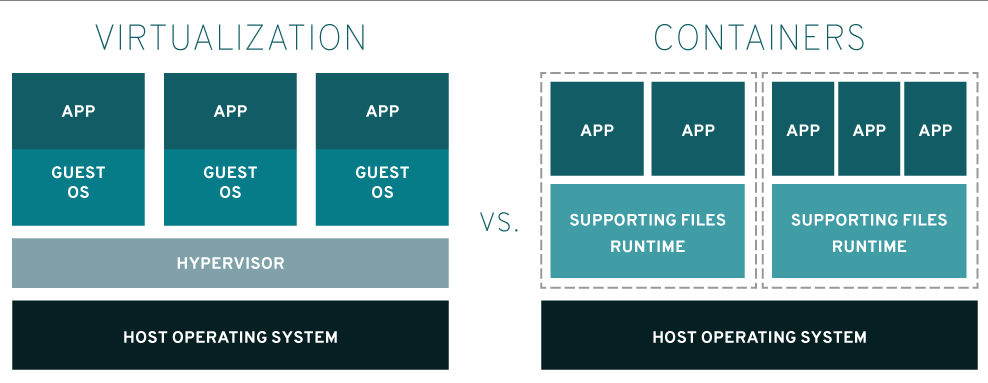
\includegraphics[scale=0.45]{Imagenes/dockervsvm1.png}
\caption{Virtualización VS Containers}
\label{dock-1}
\end{figure}

Docker, en concreto, es una plataforma que mejora el sistema LXC (proyecto de contenedores de linux) combinando este sistema con herramientas propias. Actualmente se puede ejecutar tanto en Linux como en MAC o Windows, lo que hace que cada contenedor pueda ser lanzado indistintamente de la máquina o el SO. Pero, ¿esto es del todo cierto? ¿cómo puede lanzar un contenedor de Linux en Windows o viceversa? Evidentemente, esto no es posible, en el caso de Windows, por ejemplo, la solución consiste en lanzar una maquina virtual con un kernel de Linux sobre el hyper-V (el hypervisor de windows a partir de Windows 10) o sobre una maquina virtual Virtualbox (versiones anteriores) y ejecutar todos los contenedores de Linux sobre esa máquina virtual. Sin embargo, los contenedores de Windows únicamente es posible lanzarlos desde este mismo sistema operativo \cite{Dck-10}. \par

Cada imagen del contenedor Docker se almacenan físicamente en el disco con una estructura de diferentes capas que hace que, cada imagen, sea aún más ligera de almacenar. Dicha cuestión ocurre porque se puede aplicar algo similar al concepto de herencia entre las diferentes máquinas permitiendo así, que cada imagen sea a su vez parte de la máquina de la que hereda. Para entender esto, debemos saber cuál es la estructura de un Dockerfile que define la imagen de un contenedor Docker. Cada una de estas imágenes se etiquetan con un nombre de modo que sean fáciles de manejar posteriormente.\par

Un Dockerfile es un fichero que contiene diferentes macros para compilar y crear la imagen. La primera instrucción de dicha imagen siempre es el contenedor base \cite{Dck-11}. Cada una de las instrucciones que se ejecuten da lugar a una nueva capa (layer) que se almacena y se puede compartir, si fuera necesario, entre otros contenedores. Siguiendo con el símil de los contenedores físicos, cada contenedor tiene un límite de capacidad, que en este caso es un límite de capas se pueden almacenar para un solo contenedor. Cuando se ha realizado este trabajo el límite estaba en 150 capas. \cite{Dck-12}. \par

Este diseño de capas nos permite, además de ocupar menos espacio en disco, poder tenerlas en un repositorio y solo descargarnos las capas que no tenemos. Docker nos proporciona la herramienta Docker Hub, un repositorio público similar a los repositorios de código pero que, a diferencia de estos, almacena las imágenes de los contenedores. Además, podremos descargar cualquier imagen y ejecutarla en cualquier máquina que tenga instalado Docker.\par

Por otro lado, Docker nos ofrece la herramienta “compose”. Dicha herramienta nos permite lanzar y administrar, con una sola instrucción, diversas aplicaciones y servicios de múltiples contenedores. Para ello, se define un fichero en formato YAML según la estructura definida por Docker \cite{Dck-13}. Gracias a dicha herramienta, es muy sencillo levantar y manejar toda una estructura de aplicaciones y diferentes servicios.\par

Por último, vamos a comentar por qué hemos elegido Docker frente a otras posibilidades. Aunque algunas empresas nos recomiendan subcontratar los nuevos proyectos relacionados con tecnologías de Big Data en vez de hacer un proyecto DIY (Do It Yourself) \cite{Dck-14}, dada la naturaleza de nuestro trabajo, Docker es la mejor opción. Docker nos ofrece ventajas tales como replicar y modificar las máquinas fácilmente, podemos usarlo desde cualquier máquina descargando la imagen directamente de Docker Hub y, posteriormente, poder probarlo en la nube sin tener que realizar grandes modificaciones. De esta forma, realizar cualquier cambio no requiere hacer copias de una máquina virtual entera sino modificar el Dockerfile de la máquina correspondiente. En la figura \ref{dock-2} \cite{Dck-15} podemos comprobar que el rendimiento que se obtiene con Docker es mejor que el de usar una máquina virtual KVM tanto para el arranque de las máquinas como para el benchmark UnixBench \cite{Dck-15}. En concreto, obtenemos un 30\% más de rendimiento con Docker que con KVM aunque, evidentemente, lo mejor es ejecutarlo sobre la máquina directamente. También podemos comprobar en la figura \ref{dock-3}  \cite{Dck-15} que el tiempo que tarda en arrancar una máquina Docker es de 5 segundos, mientras que una máquina virtual KVM tarda 15 segundos.\par

\begin{figure}[htp]
\centering
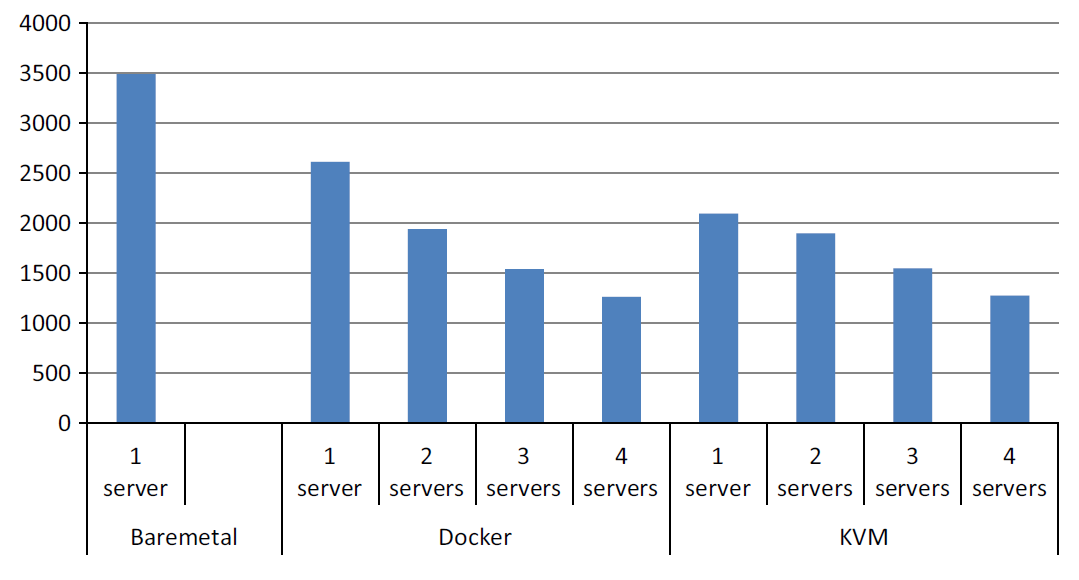
\includegraphics[scale=0.40]{Imagenes/dockervsvm2.png}
\caption{Rendimiento del benchmark con el índice UnixBench para el software sobre una máquina real, sobre Docker y sobre KVM}
\label{dock-2}
\end{figure}

\begin{figure}[htp]
\centering
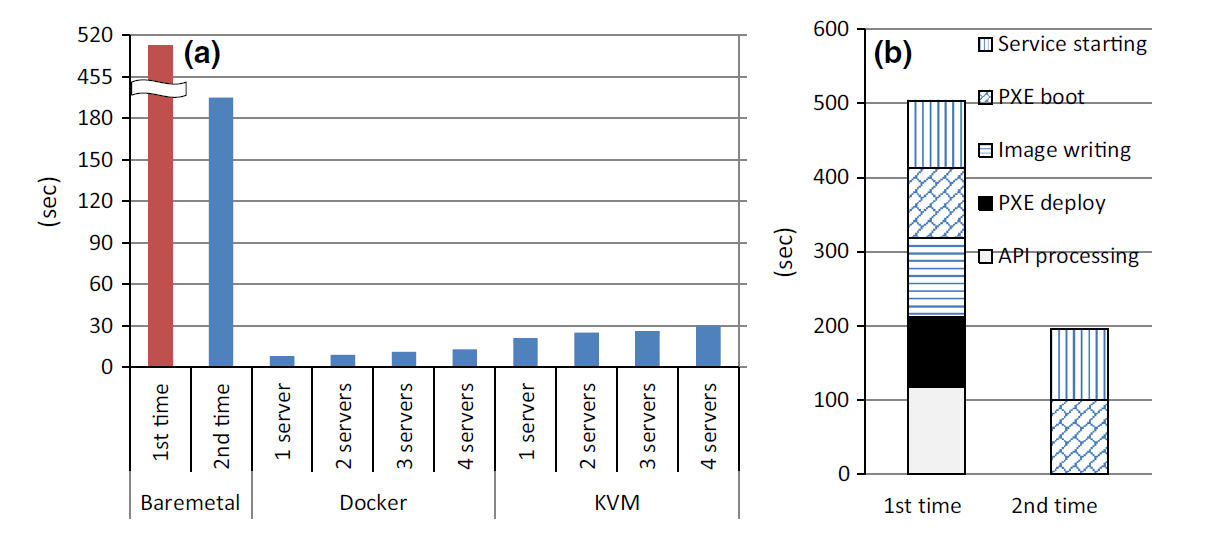
\includegraphics[scale=0.40]{Imagenes/dockervsvm3.png}
\caption{Tiempo de arranque sobre una máquina real, sobre Docker y sobre KVM}
\label{dock-3}
\end{figure}


\subsection{Apache Hadoop\label{Hadoop}}



Obviamente, cuando hablamos de Big Data tenemos que hacer referencia a Apache Hadoop. Para la realización de esta herramienta, se basaron en dos en dos artículos publicados por Google sobre su sistema de ficheros distribuido \cite{Hdp-2} y MapReduce \cite{Hdp-3}. El sistema de ficheros de Hadoop fué bautizado como HDFS convirtiéndose en una herramienta muy popular de la que hacen uso grandes empresas como Yahoo!,   Last.fm, Facebook o el New York Times. Además de esto, en 2009, Hadoop superó el récord de Google en ordenar un terabyte de datos en menos tiempo \cite{Hdp-1}. Además de esto, Apache Hadoop forma parte de Apache Foundation, lo que quiere decir que es totalmente OpenSource.\par

Actualmente, la arquitectura de la versión 3 de Hadoop, está formada por cuatro módulos principales y sus diferentes servicios \cite{Hdp-4}:\par

\begin{itemize}
	\item \textbf{Hadoop Common}: Este paquete contiene las utilidades comunes que soportan todos los demás módulos de Hadoop.
	\item \textbf{Hadoop Distributed File System (HDFS)}: Es el sistema de ficheros distribuido de Hadoop. Por definición es un sistema de ficheros distribuidos que proporciona un alto rendimiento a los datos de aplicación. Tiene una estructura maestro/esclavo que se compone de los siguientes servicios:
	\begin{itemize}
		\item \textbf{Namenode}: Administra el espacio de nombres del sistema de ficheros y regula el acceso a los diferentes ficheros. Además, asigna el datanode donde se almacenará cada bloque físico de cada fichero para que quede balanceado dicho sistema. Por tanto, en este nodo se encontrarán los metadatos de donde se encuentra cada bloque.
		\item \textbf{Datanode}: Es un nodo de almacenamiento. En dicho nodo existirán bloques de datos, asignados por el NameNode.
		\item \textbf{Secondary NameNode}: Es una réplica del namenode que se usa como copia por si en algún momento el NameNode cae. Se hace una copia de los metadatos cada hora o cada millón de transacciones por defecto.
		\item \textbf{Checkpoint node}: Al igual que el Secundary NameNode, hace copias de seguridad del NameNode, pero no tiene la capacidad de sustituirlo.
	\end{itemize}
	\item \textbf{Hadoop YARN}: Este módulo es el framework que gestiona los trabajos y los diferentes recursos del cluster. La idea consiste en separar la planificación y la supervisión de los diferentes trabajos sobre Hadoop. También usa una estructura de maestro/esclavo para los cuales se suministran los siguientes servicios:
	\begin{itemize}
		\item \textbf{Resource Manager}: Este servicio se considera el “maestro”. Tiene dos funcionalidades principales, la función de Scheduler (planificador) y la función de ApplicationsManager (gestor de aplicaciones). Como planificador debe ser capaz de asignar los recursos necesarios a cada aplicación cuando lo necesite o reiniciar una aplicación en caso de fallo. Como gestor de aplicaciones es el encargado de asignar trabajo a cada uno de los componentes del cluster.
		\item \textbf{Node Manager}:Es el responsable de iniciar y administrar los trabajos para una nodo del cluster.
		\item \textbf{ProxyServer}: Por defecto, se ejecuta junto al Resource Manager, pero se puede ejecutar por separado. Se encarga de reducir ataques web que puedan producirse a través de YARN.
	\end{itemize}
	\item \textbf{Hadoop MapReduce}: Es el módulo para el procesamiento paralelo de grandes conjuntos de datos. Este sistema está basado en YARN. Además, tiene un servicio adicional que podemos añadir: 
	\begin{itemize}
		\item \textbf{HistoryServer}: simplemente muestra a través de una web los logs que producen los diferentes trabajos de MapReduce.
	\end{itemize}
\end{itemize}

HDFS, como ya hemos dicho, es el sistema de ficheros de Hadoop, cuya característica más importante es que es distribuido, aunque no es la única característica que posee. HDFS, como los sistemas de ficheros convencionales, distribuye los diferentes ficheros en bloques de un tamaño fijo, normalmente de 128 MB, ya que suponen ficheros de gran tamaño, aunque esto es modificable. Dichos bloques están divididos entre los diferentes nodos del cluster de forma que sea más fácil realizar diversos tratamientos sobre ellos de forma paralela. Además de esto, contamos con la replicación de los distintos bloques, según establezcamos cuantas replicaciones de bloque queramos. Esto tiene muchas implicaciones tales como cuando cae uno de los nodos, siempre tenemos los datos disponibles en otro nodo, si uno de los nodos cae o se rompe el disco duro, podemos volver a generar dicho nodo a partir de los metadatos del namenode y la replicación de bloques. Dicho esto, podemos ver que no tiene sentido montar un RAID sobre el servidor, ya que el sistema de Hadoop te proporciona dicha funcionalidad.\par

MapReduce consiste en uno o varios procesos distribuidos que manejan grandes volúmenes de datos. Tiene dos funciones principales, map y reduce. La función Map genera una tupla clave/valor intermedios y la función Reduce combina esos valores para cada clave para obtener un resultado. Dicho esto, se muestra en la figura \ref{hdImg1} \cite{Hdp-1} un ejemplo de cómo funcionaria gráficamente:\par

\begin{figure}[htp]
\centering
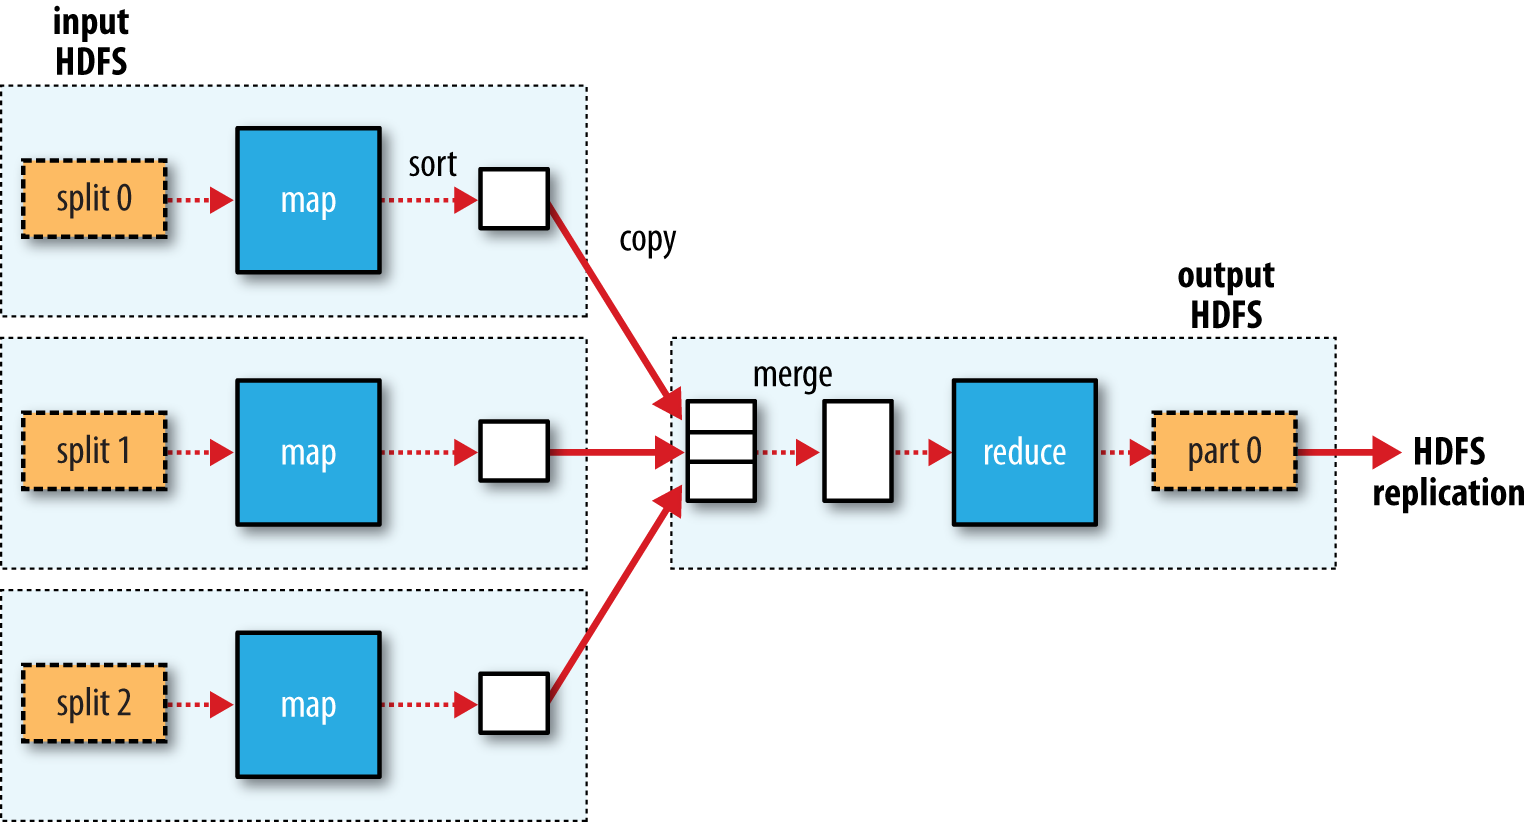
\includegraphics[scale=0.28]{Imagenes/hadoop1.png}
\caption{Funcionamiento de Map Reduce sobre HDFS. }
\label{hdImg1}
\end{figure}

Por último, decir que Apache Hadoop está programado en Java y necesitamos la JVM (Java Virtual Machine) para ejecutarlo.\par


\subsection{Apache Spark\label{Spark}}
\subsection{Apache Kafka\label{Kafka}}
\subsection{Elastic\label{Elastic}}
\subsection{MongoDB\label{MongoDB}}
